\chapter{Entwicklung eines GraphQL-Service in .NET mit HotChocolate}
In diesem Kapitel wird die prototypische Entwicklung eines GraphQL-Service beschrieben.
Der Prototyp wurde mit .NET 6 und unter Zuhilfenahme der Bibilothek HotChocolate entwickelt wurde.

\section{Anwendungsszenario}
% Der Anwendungsfall des Prototypen lässt sich wie folgt beschreiben:
% Da die Verwaltungen von Büchern und dazugehörige Autoren und Bewertungen ein aufwändiges Verfahren ist soll 
Die Auswahl eines neuen Buches ist oftmals ein sehr schwieriges Unterfangen.
Bei der Entscheidungsfindung helfen oft Bewertungen von Kunden, die das jeweilige Buch schon gelesen haben.
Daher soll eine Bücher-Bewertungsplattform geschaffen werden.
Diese Plattform ermöglicht es Benutzern, Bücher zu bewerten und Informationen über Bücher, Autoren oder Bewertungen einzusehen.
% Benutzer, mit mehr Rechten als reinen Benutzerrechen, haben zudem die Möglichkeit die zusätzlich benötigten Entitäten 
Weiters sollen Benutzer in der Lage sein, sich im System zu registrieren und anzumelden.
Angemeldete Benutzer haben, je nach ihren Benutzerrollen, Möglichkeiten, im System verwaltete Entitäten zu erstellen, zu bearbeiten oder zu löschen.

\section{Design der Schnittstelle}
Bevor ein Entwickler sich um die technische Umsetzung einer API kümmert, ist es ratsam, dass er sich einen Gesamtüberblick über das zu entwerfende System verschafft.
Dafür werden vor Beginn der technischen Umsetzung auf Grundlage des Anwendungsszenarios, Anwendungsfälle definiert.
% Diese Use-Cases definieren die Art und Weise wie ein Client auf den GraphQL-Service zugreif.
Diese Anwendungsfälle beschreiben die benötigten Zugriffe eines Clients auf das System.
% Mit diesen Use-Cases definiert man wie ein Client auf den zukünftigen GraphQL-Service zugreift.
Zudem werden mit der Definition der Zugriffe auch die benötigen Entitäten definiert.
% Weiters erfolgt eine erste Definition der zu verwaltenden Objekte.
Aus dem Anwendungsszenario abgeleitete Use-Cases werden in der folgenden Abbildung grafisch dargestellt:

\begin{figure}[H]
    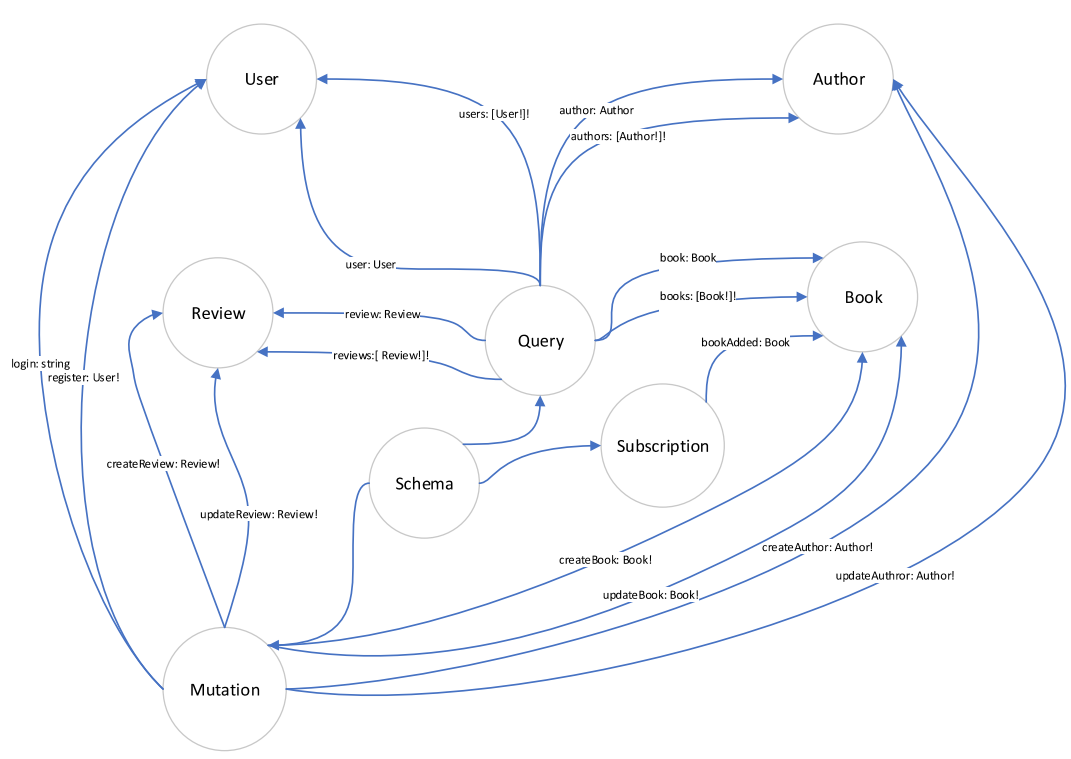
\includegraphics[width=\textwidth]{pics/graph_usecases.png}
    \caption{Use-Cases für das Beispielszenario.}
\end{figure}

Die obige Abbildung beschreibt die Zugriffsmöglichkeiten eines Clients auf den Prototypen.
Mit der Definition der Use-Cases geht auch die Definition der erforderlichen Entitäten einher.
Die erforderlichen Entitäten und ihre Relationen zueinander sind im folgenden ER-Diagram dargestellt:
% Weiters sind die Entitäten auf die Zugriffe möglich sind abgebildet.
% Dabei werden die Zugriffe jeweils
% Weiters zeigen die Use-Cases welche Entitäten im System zur Verfügung stehen werden.

% In der gezeigten Abbildung sieht man die vom Prototypen verwalteten Entitäten.
% Ebenso werden die lesenden und schreibenden Operationen auf diese dargestellt.

% Die zu verwaltenden  Relationen zwischen den Entitäten sind im folgenden ER-Diagram dargestellt:
\begin{figure}[H]
    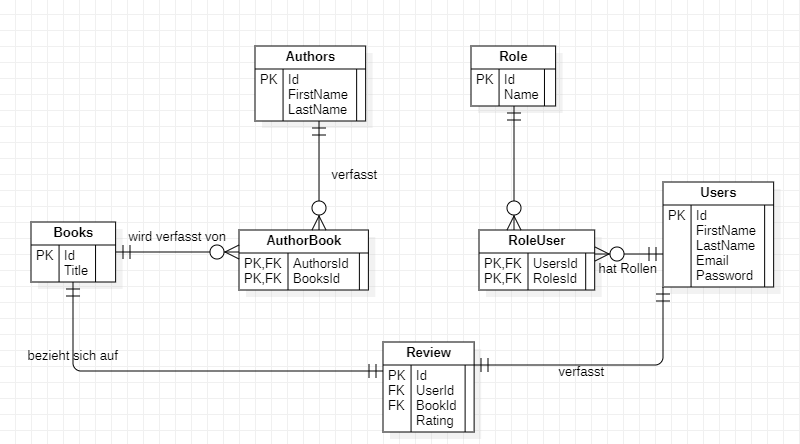
\includegraphics[width=\textwidth]{pics/ER-Diagram.png}
    \caption{Datenbankschema}
\end{figure}

\section{HotChocolate}
Für die Implementierung des GraphQL-Service wurde das Framework HotChocolate herangezogen.
Neben HotChocolate wird auch noch das Framework .NET GraphQL häufig eingesetzt.
% Der Prototyp wurde aufgrund der steigenden Beliebtheit und Aktivät der Community des HotChocolate Frameworks mit eben jenem Framework umgesetzt.
Die Entscheidung fiel auf HotChocolate aufgrund der besseren Dokumentation des Frameworks und der höheren Aktivität der Community.

\myparagraph{HotChocolate allgemein} %TODO allgemein umbennen vielleicht auf generell
HotChoclate ist ein quelloffenes Framework zur Implementierung eines GraphQL-Service.
Es ist konform zur GraphQL-Spezifikation implementiert.
Damit ist HotChocolate kompatibel mit allen GraphQL konformen Clients.
Der Entwurf des Schemas gehört zu den Kernaufgaben bei der Entwicklung eines GraphQL-Service.
% Ein großer Teil der Komplexität, einen GraphQL-Service zu entwickeln, fällt dabei auf die Entwicklung des Schemas zurück.
% HotChoclate kümmert sich um die Generierung des Schemas zur Laufzeit und entfernt somit einen großen Teil dieser Komplexität vom Entwickler.

\myparagraph{Schema-Erstellung in HotChocolate}
Es gibt drei Varianten, in HotChoclate ein Schema zu entwickeln: \textit{Pure-Code-First}, \textit{Code-First} und \textit{Schema-First}.
Schema-First übernimmt dabei ein bereits bestehendes Schema und fügt es dem Service zu.
Code-First verwendet Attribute um das Schema zu definieren.
Pure-Code-First verwendet eine Fluent-API.
Alle drei Varianten liefern dasselbe Schema, wobei man mit Pure-Code-First-Ansatz am meisten Kontrolle bei der Konfiguration hat.
Der Prototyp wurde mittels der Pure-Code-First-Vorgehensweise umgesetzt.

\myparagraph{Abhängigkeitsinjektion}
Abhängigkeitsinjektion in HotChocolate funktioniert sehr ähnlich wie die Abhängigkeitsinjektion von ASP.NET-Applikationen.
Die Services werden, so wie die anderen Komponenten der Anwendung, zum Service-Container hinzugefügt:

\begin{JsCode}
builder.Services.AddTransient(typeof(IRepository<>), typeof(Repository<>));
builder.Services.AddTransient(typeof(IBookRepository), typeof(BookRepository));
builder.Services.AddTransient(typeof(IAuthorRepository), typeof(AuthorRepository));
builder.Services.AddTransient(typeof(IReviewRepository), typeof(ReviewRepository));
builder.Services.AddTransient(typeof(IBaseService<>), typeof(BaseService<>));
builder.Services.AddTransient<IBookService, BookService>();
builder.Services.AddTransient<IAuthorService, AuthorService>();
builder.Services.AddTransient<IReviewService, ReviewService>();
builder.Services.AddTransient<IAuthService, AuthService>();
\end{JsCode}

HotChocolate unterstüzt aber nicht die Konstruktor-Injektion.
Stattdessen wird die Abhängigkeitsinjektion in HotChoclate mittels Methoden-Injektion umgesetzt.
Würde man die Abhängigkeitsinjektion mittels Konstruktor-Injektion implementieren, wäre jeder Service automatisch ein Singleton.
Für die Methoden-Injektion liefert HotChocolate das Attribute [Service].

Im folgenden Quelltextausschnitt ist ersichtlich, wie Methoden-Injektion verwendet wird:
\begin{JsCode}
public async Task<IQueryable<Book>> Books([Service]IBookService bookService)
{
    //Execute logic here
}
\end{JsCode}

\section{Architektur}
Der Prototyp wurde mit der für REST-APIs üblichen Drei-Schicht-Architektur umgesetzt.
Die Geschäftslogikschicht und Datenbankzugriffsschicht wurden laut dem \textit{Program to an Interface not an Implementation}-Prinzip entwickelt, somit können die konkreten Implementierungen, je nach Bedarf, einfach ausgetauscht werden.
% Auf die Geschäftslogik wird in den Unterkapiteln Query, Mutation und Subscription näher eingegangen. Die Datenbankzugriffsschicht wird im Kapitel Entity Framework näher erläutert.
\newline

\begin{figure}[H]
    \centering
    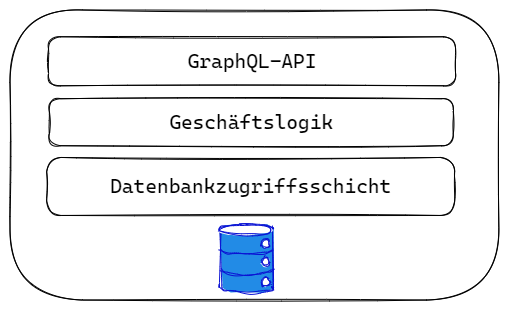
\includegraphics[width=0.5\textwidth]{pics/architecture.png}
    \caption{Drei-Schicht-Architektur}
\end{figure}

Abb 4.4. gibt einen Überblick über die Gesamtarchitektur.
Die gezeigten Schichten werden in den folgenden Abschnitten näher erläutert.

\subsection{API:}
Die API bildet die einzige Schnittstelle des Systems zur Außenwelt.
Sie ist ein Abbild des GraphQL-Schemas.
Dieses Schema definiert, wie in Abschnitt 3.3 beschrieben, die verfügbaren Typen sowie die lesenden und schreibenden Zugriffe des GraphQL-Service.

\subsection{Geschäftslogik}
% Die Geschäftslogik bildet dabei die Logik der Server-Applikation ab.
Die Geschäftslogik wird dem GraphQL-Schema mittels Resolvern zur Verfügung gestellt.
Genaueres zu den Resolvern und zur Geschäftslogik folgt im Abschnitt 4.5.
Die Geschäftslogik besteht aus \textit{Service}-Klassen und zugehörigen Interfaces welche mit der Datenbankzugriffsschicht interagieren.

\subsection{Datenbankzugriff}
Die darunterliegende Datenbankzugriffsschicht ermöglicht den darüberliegenden Schichten CRUD-Operationen auf die angeforderten Daten auszuführen.
Für die Datenbankzugriffsschicht wurde dabei das Entity Framework verwendet.
Das Entity Framework ist ein \textit{Object Relational Mapper}, der es Entwicklern ermöglicht, den Fokus auf eine höhere Abstraktionsebene zu legen.
Diese Schicht wurde mit dem Repository-Pattern umgesetzt.
Ein generisches Repository stellt die Grundfunktionalität für die anderen entitätsspezifischen Repositories zur Verfügung.
Der folgende Quelltextausschnitt zeigt einen Teil der Implementierung der Grundfunktionalitäten:
\begin{JsCode}
public class Repository<TEntity> : IRepository<TEntity> where TEntity : BaseEntity {
    protected readonly LibraryContext context;
    public Repository(IDbContextFactory<LibraryContext> contextFactory) {
        this.context = contextFactory.CreateDbContext();
    }

    public async Task<IQueryable<TEntity>> GetAsync(Expression<Func<TEntity, bool>> filter = null, params Expression<Func<TEntity, object>>[] includes) {
        IQueryable<TEntity> query = context.Set<TEntity>();

        foreach (var include in includes) {
            query = query.Include(include);
        }

        if (filter != null) {
            query = query.Where(filter);
        }

        return query.AsQueryable();
    }

    public virtual async Task<TEntity> AddAsync(TEntity entity) {
        if (entity is null) {
            throw new ArgumentNullException(nameof(entity));
        }

        await context.AddAsync(entity);
        await context.SaveChangesAsync();
        return entity;
    }

    public virtual async Task<TEntity> UpdateAsync(TEntity entity) {
        if (entity is null) {
            throw new ArgumentNullException(nameof(entity));
        }

        context.Entry(entity).State = EntityState.Modified;

        await context.SaveChangesAsync();
        return entity;
    }
}
\end{JsCode}

Im folgenden Quelltextausschnitt wird die Implementierung des Repository für die Domänenklasse Book gezeigt.
Es zeigt die notwendigen Überschreibungen der Basisimplementierung:

\begin{JsCode}
public class BookRepository : Repository<Book>, IBookRepository {
    public BookRepository(IDbContextFactory<LibraryContext> contextFactory)
        : base(contextFactory) { }

    public override async Task<Book> AddAsync(Book book) {
        book.Authors = await context.Authors
            .Where(author => book.Authors.Select(x => x.Id)
            .ToList().Contains(author.Id)).ToListAsync();
        return await base.AddAsync(book);
    }

    public override async Task<Book> UpdateAsync(Book book) {
        var bookToUpdate = await GetFirstAsync(
            b => b.Id == book.Id, b => b.Authors);
        if (bookToUpdate == null) {
            throw new ArgumentNullException(nameof(bookToUpdate));
        }

        bookToUpdate.Title = book.Title;

        if (book.Authors.Count != bookToUpdate.Authors.Count
            || !bookToUpdate.Authors.All(book.Authors.Contains))
        {
            bookToUpdate.Authors.UpdateManyToMany(book.Authors, b => b.Id);
            bookToUpdate.Authors = await context.Authors
            .Where(author => book.Authors.Select(a => a.Id)
                            .ToList().Contains(author.Id))
                            .ToListAsync();
        }

        return await base.UpdateAsync(bookToUpdate);
    }
}
\end{JsCode}

\section{Resolver}
Das Schema beschreibt, wie in Abschnitt 3.3 erwähnt, nur die verfügbaren Typen, Querys, Mutations und Subscriptions.
% Über die Generierung der Daten als auch über die Manipulation dieser hat das Schema kein Wissen.
Aus dem Schema ist aber die Generierung der Daten als auch die Manipulation dieser nicht abbildbar.
Für den Datenzugriff bzw. Datenmanipulation sind in GraphQL \textit{Resolver} verantwortlich.
Jedes Feld in einer Query ist nichts anderes als eine Methode, welches den Wert dieses Typs retourniert.
Jedes Feld eines Typs wird dabei einem \textit{Resolver} zugewiesen, diese Resolver sind Zugriffe auf die Geschäftslogik.
Wird ein Feld durch eine Query angefordert, liefert der jeweilige \textit{Resolver} die angeforderten Daten zurück.

\myparagraph{Umsetzung Resolver}
Resolver delegieren im Prototyp an entsprechende Methoden der Geschäftslogik, welche CRUD-Operationen der jeweiligen Entität zur Verfügung stellt.
% Resolver werden im Prototypen durch die Geschäftslogik abgebildet, diese bieten CRUD-Operationen für die jeweilige Entität.
Jede Entität verfügt über einen \textit{Service}.
Jeder Service, wie zum Beispiel der \textit{AuthorService}, leitet von einem generisch implementierten \textit{BaseService} ab.
Der \textit{BaseService} implementiert dabei das Interface \textit{IBaseService}.
% Diese Services werden durch ein generisches \textit{Interface} \textit{IBaseService} und eine generische Basisimplementierung \textit{IBaseService} definiert.
\newline

\begin{JsCode}
public interface IBaseService<TEntity> where TEntity: BaseEntity {
    public Task<IQueryable<TEntity>> GetAsync(Expression<Func<TEntity, bool>> filter = null, params Expression<Func<TEntity, object>>[] includes);
    public Task<TEntity> GetFirstAsync(Expression<Func<TEntity, bool>> filter = null, params Expression<Func<TEntity, object>>[] includes);
    public Task<TEntity> AddAsync(TEntity entity);
    public Task<TEntity> UpdateAsync(TEntity entity);
    public Task<bool> ExistsAsync(int id);
    public Task RemoveAsync(TEntity entity);
}
\end{JsCode}

Im obigen Quelltextausschnitt ist das generische Interface \textit{IBaseService} abgebildet.
Es bietet Schnittstellen für die CRUD-Operationen jeder Entität.

\begin{JsCode}
public class BaseService<TEntity> : IBaseService<TEntity> where TEntity : BaseEntity {
    protected readonly IRepository<TEntity> repository;

    public BaseService(IRepository<TEntity> repository) {
        this.repository = repository;
    }
    public virtual async Task<IQueryable<TEntity>> GetAsync(Expression<Func<TEntity, bool>> filter = null, params Expression<Func<TEntity, object>>[] includes) {
        return await repository.GetAsync(filter, includes);
    }

    public virtual async Task<TEntity> GetFirstAsync(Expression<Func<TEntity, bool>> filter = null, params Expression<Func<TEntity, object>>[] includes) {
        return await repository.GetFirstAsync(filter, includes);
    }

    public virtual Task<TEntity> AddAsync(TEntity entity) {
        return repository.AddAsync(entity);
    }
    public virtual async Task<TEntity> UpdateAsync(TEntity entity) {
        return await repository.UpdateAsync(entity);
    }

    public virtual async Task<bool> ExistsAsync(int id) {
        return await repository.ExistsAsync(id);
    }

    public virtual async Task RemoveAsync(TEntity entity) {
        await repository.RemoveAsync(entity);
    }
}
\end{JsCode}

Im obigen Quelltextausschnitt ist die Basisimplementierung jedes Service zu sehen.
Besonders relevant für das Zusammenspiel mit HotChocolate ist dabei, dass die lesenden Operationen ein \textit{IQueryable} zurückliefern.
Warum IQueryable so wichtig ist für HotChocolate wird im Abschnitt 4.6 näher erläutert.

%TODO Aufrufe relevant pagination -> projection -> filtering -> sorting
%todo die absätze aufeinander abstimmen erwähnen dass nur sortiert werden kann nachdem gefiltert wurde usw... bis nach oben hin
%sorting, filtering, projection ist ja nichts anders als middelware die nacheinander exekutiert wird, dabei Grafik von HotChocolate verwenden zur Veranschaulichung
\section{Field Middleware}
Field-Middleware erlaubt es, wiederverwendbare Logik vor oder nach der Ausführung des Resolvers auszuführen.
% Diese Funktionalitäten sind Field-Middleware Komponenten von HotChocolate.
Funktionalitäten wie Authentifizierung / Autorisierung, Sortieren, Filtern, Pagination und Projektionen werden dabei von HotChocolate als Middleware-Komponenten zur Verfügung gestellt. 
Man kann beliebig viele Middleware-Komponenten aneinanderreihen.
Sie sind eine der fundamentalen Komponenten des Frameworks.

% Im folgenden Unterkapitel Query werden Funktionalitäten für das Authentifizieren und Autorisieren eines Benutzers als auch für das Sortieren, dem Filtern und der Projection verwendet.

\myparagraph{Reihenfolge Exekution Middleware}
Jede Middleware-Schicht kennt nur die jeweils nächste Middleware.
Die letzte auszuführende Middleware ist der eigentliche Resolver.
Die Reihenfolge der Anordnung der Middleware-Komponenten ist dabei sehr entscheidend, denn die Komponenten werden in genau dieser Reihenfolge ausgeführt.
% Die Reihenfolge in der diese Middlewarekomponenten ausgeführt werden ist dabei sehr wichtig, denn sie entscheidet in welcher 
Die folgende Abbildung beschreibt die Aneinanderreihung der Middleware-Komponenten:

\begin{figure}[H]
    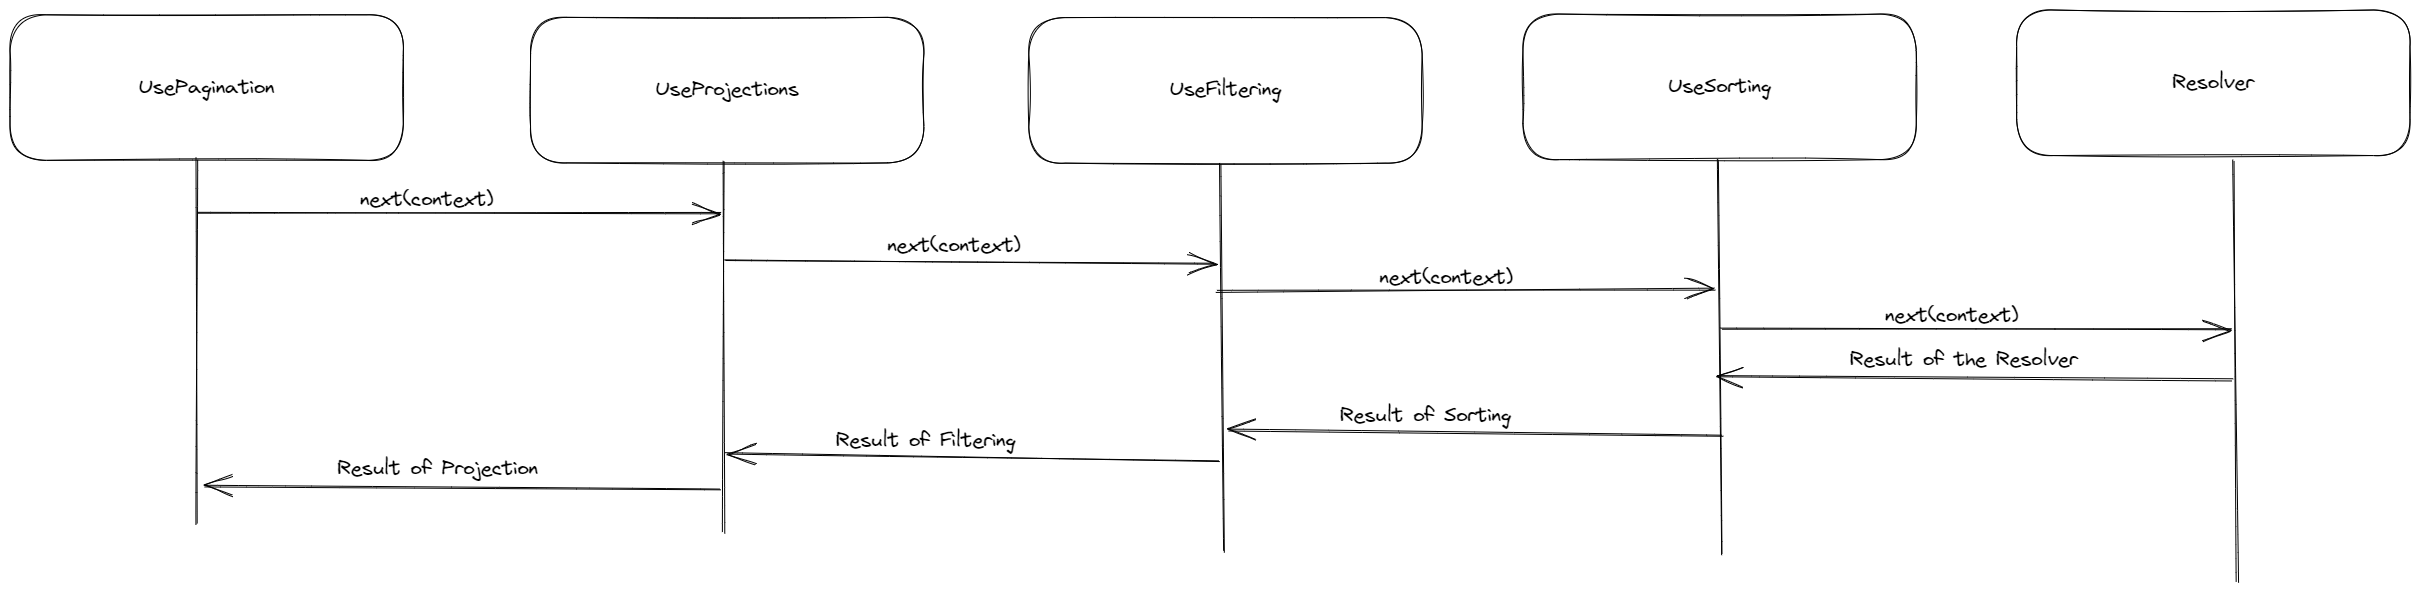
\includegraphics[width=\textwidth]{pics/middleware.png}
    \caption{Ausführungsreihenfolge Middleware}
\end{figure}

In der obigen Abbildung ist zu sehen, dass die Middleware in der Reihenfolge ausgeführt wird, in der sie definiert wurde.
Das Resultat, welches von der letzten Middleware (dem Resolver) generiert wurde, wird in der umgekehrten Reihenfolge zurückgereicht.
Dabei wird das vom Resolver zurückgelieferte \textit{IQueryable} um die jeweiligen Operationen der restlichen Middleware-Komponenten erweitert.
\newline

Im Abschnitt 4.7 werden die verwendeten Middleware-Komponenten des Prototypen genauer erläutert.
% Da im Unterkapitel Query, welche die in der Implementierung, diese Middlewarekomponenten verwendet werden, erfolgt dort auch eine genauere Erläuterung der einzelnen Komponenten.
% In den folgenden Abschnitten wird auf zuvor erwähnten Middlewarekomponenten genauer eingegangen, diese sind für die folgenden Unterkapitel Query und Mutation von besonderer Relevanz: 

\myparagraph{Ausführung Middleware}
Nachdem jene Middleware, welche als erstes definiert wurde, das Ergebnis der restlichen Middleware-Komponenten erhalten hat, wird die \textit{LINQ}-Abfrage ausgeführt und das Ergebnis an den Client zurückgeliefert.

\section{Querys}
Im folgenden Abschnitt wird die Umsetzung eines lesenden Zugriffs mittels einer Query auf die Entität \textit{Author} erläutert.
Dabei wird das Zustandekommen der Schema-Definition der Query als auch der Zugriff auf die Datenbank mittels der Geschäftslogik eingegangen.
Weiters wird erläutert wie HotChocolate das Problem des Over- und Underfetchings löst und Filtern, Sortieren und Pagination ermöglicht.
\newline
Die folgenden Unterabschnitte widmen sich der Umsetzung der Query authors welche alle im System gespeicherten Autoren liefert.
Dabei kann man diese Entitäten filtern, sortieren und paginieren. %TODO --> paginieren nicht so nice i guess

\myparagraph{Generierung Schema}
Um es einem Client zu ermöglichen, auf die Autoren zuzugreifen, ist es erforderlich, die Query im Schema zu definieren.
Hierbei wird für die Generierung des Schemas der bereits erwähnte Pure-Code-First-Ansatz verwendet.
\newline

\begin{JsCode}
public class AuthorQuery: ObjectType<Query> {
  protected override void Configure(IObjectTypeDescriptor<Query> descriptor){
    descriptor.Field("authors")
        .ResolveWith<AuthorResolver>(r => r.Authors())
        .Authorize()
        .UseProjection()
        .UseFiltering()
        .UseSorting()
        .Type<ListType<NonNullType<AuthorType>>>();
   }
}
\end{JsCode}

Im obigen Quelltextausschnitt ist zu sehen, dass die Wurzeloperation vom Typ ObjectType$<Query>$  um AuthorQuery erweitert wird.
Überschreibt man nun die in der Klasse ObjectType definierte Methode Configure, kann man die Felder der Query mit dem IObjectTypeDescriptor erweitern.
Dabei wird das Feld \textit{authors} angelegt, welches eine Liste von Autoren zurückgibt.
Die angeforderten Daten des Clients werden vom Resolver zur Verfügung gestellt.
Resolver werden im Abschnitt 4.5 näher eräutert.
\newline

In den folgenden Quelltextausschnitten wird das zur Laufzeit generierte Schema gezeigt:
\begin{JsCode}
type Query{
    authors(where: AuthorFilterInput order: [AuthorSortInput!]): [Author!] @authorize(apply: BEFORE_RESOLVER)
}

type Author {
    firstName: String!
    lastName: String!
    books: [Book!]!
    id: Int!
}
\end{JsCode}

Nur der Objekt-Typ \textit{Author} als auch die Wurzel-Operation der Query mit dem Feld \textit{authors} wurden explizit generiert.
% Die restlichen, im folgenden Code-Beispiel gezeigten Objekt-Typen wurden durch die aufgerufenen Middleware-Komponenten implizit generiert:
Die Methodenaufrufe \textit{Authorize()}, \textit{UseFiltering()} und \textit{UseSorting()} sind für die implizite Generierung, der im nachfolgenden Schema angegebenen Typen, verantwortlich.
Diese Methodenaufrufe aktivieren die jeweilige Field-Middleware, diese werden in den nachfolgenden Abschnitten genauer erläutert.

\begin{JsCode}
input AuthorFilterInput {
    and: [AuthorFilterInput!]
    or: [AuthorFilterInput!]
    firstName: StringOperationFilterInput
    lastName: StringOperationFilterInput
    books: ListFilterInputTypeOfBookFilterInput
    id: ComparableInt32OperationFilterInput
}

input ListFilterInputTypeOfBookFilterInput {
  all: BookFilterInput
  none: BookFilterInput
  some: BookFilterInput
  any: Boolean
}

input AuthorSortInput {
    firstName: SortEnumType
    lastName: SortEnumType
    id: SortEnumType
}

input StringOperationFilterInput {
  and: [StringOperationFilterInput!]
  or: [StringOperationFilterInput!]
  eq: String
  neq: String
  contains: String
  ncontains: String
  in: [String]
  nin: [String]
  startsWith: String
  nstartsWith: String
  endsWith: String
  nendsWith: String
}

input ComparableInt32OperationFilterInput {
    eq: Int
    neq: Int
    in: [Int!]
    nin: [Int!]
    gt: Int
    ngt: Int
    gte: Int
    ngte: Int
    lt: Int
    nlt: Int
    lte: Int
    nlte: Int
}
\end{JsCode}

\myparagraph{Authorize}
Hierbei wird deklariert, dass nur angemeldete Benutzer Zugriff auf dieses Feld haben.
Diese Middleware ist, wie in der obigen Schemadefinition ersichtlich, vor dem Resolver auszuführen.
Sie stellt damit sicher, dass nur Anfragen mit einer gültigen Authentifizierung an die Geschäftslogik weitergereicht werden.
Im Schema wird das Feld \textit{authors} der Query mit der Direktive @Authorize versehen.
Näheres zur Authentifizierung und Autorisierung ist im Abschnitt 4.10 ersichtlich.

\myparagraph{Projektionen}
Mit Projektionen liefert HotChocolate die Möglichkeit Over- und Underfetching zu verhindern.
Das bedeutet, dass genau jene Daten, welche vom Client angefordert werden, in der Datenbank selektiert und anschließend an den Client zurückgeliefert werden.
Dazu muss der Resolver ein Abfrageobjekt vom Typ IQueryable aber an das Framework übergeben.
% Dabei bekommt HotChocolate vom \textit{Resolver} ein \textit{IQueryable}.
Dieses Abfrageobjekt beinhaltet zunächst nur jene Filterungen und Selektionen, welche von der Geschäftslogik festgelegt werden.
HotChocolate erweitert dieses Abfrageobjekt nun durch jene Felder welche in der Query angefordert wurden.

\myparagraph{Filtering}
Aktiviert man die \textit{Filtering}-Middleware für ein Query-Field, so kann man den implizit von HotChocolate bereitgestellten Filter-Input verwenden.
Diese Middleware erweitert vom Resolver zurückgelieferte Abfrageobjekt um die gegebene Filterung und liefert das Ergebnis der vorangestellten Middleware zurück.
Im obigen Quelltextausschnitt ist ersichtlich, dass die Filtering-Middleware zur Laufzeit das Input-Objekt AuthorFilterInput und die darin referenzierten Input-Objekte generiert.
Weiters ist es möglich benutzerdefinierte Typen für die Filterung zu definieren.

\myparagraph{Sorting}
Aktiviert man die \textit{Sorting}-Middleware für ein Query-Field, so kann man den implizit von HotChocolate bereitgestellten Sortier-Input verwenden.
Diese Middleware fügt vom Resolver zurückgelieferten Abfrageobjekt die gegebene Sortierung hinzu.
Das Ergebnis wird wiederum an die vorangestellte Middleware zurückgeliefert.
Weiters ist es möglich benutzerdefinierte Typen für die Sortierung zu definieren.

\myparagraph{Zugriff auf Daten}
Der \textit{AuthorResolver} greift dabei auf die Geschäftslogik zu.
Er greift auf den AuthorService, einer Kindklasse von BaseService, zu und dieser mithilfe der Datenbankzugriffsschicht auf die Datenbank.
Wichtig dabei ist, dass der AuthorService, HotChocolate ein Abfrageobjekt zurückliefert.
Das zurückgelieferte Abfrageobjekt wird vom Resolver an die restlichen Middleware-Komponenten zurückgereicht.
Diese erweitern dann das Abfrageobjekt mit der von ihnen definierten Logik und werten es anschließend aus.
Der AuthorResolver ist im folgenden Quelltextausschnitt ersichtlich:
\begin{JsCode}
public class AuthorResolver {
    private readonly IAuthorService authorService;
    private readonly IMapper mapper;

    public AuthorResolver(IAuthorService authorService, IMapper mapper) {
        this.authorService = authorService;
        this.mapper = mapper;
    }

    public async Task<IQueryable<Author>> Authors() {
        return await authorService.GetAsync();
    }

    public async Task<Author> CreateAuthor([Service] IAuthorService authorService, AuthorCreate input) {
        return await authorService.AddAsync(mapper.Map<Author>(input));
    }

    public async Task<Author> UpdateAuthor([Service] IAuthorService authorService, AuthorUpdate input) {
        return await authorService.UpdateAsync(mapper.Map<Author>(input));
    }

    public async Task<Author> AuthorByDataLoader(int id, AuthorByIdDataLoader dataLoader, CancellationToken cancellationToken) {
        return await dataLoader.LoadAsync(id, cancellationToken);
    }
}
\end{JsCode}
\pagebreak
\myparagraph{Ausführung Query und Ergebnis}
\begin{figure}[H]
    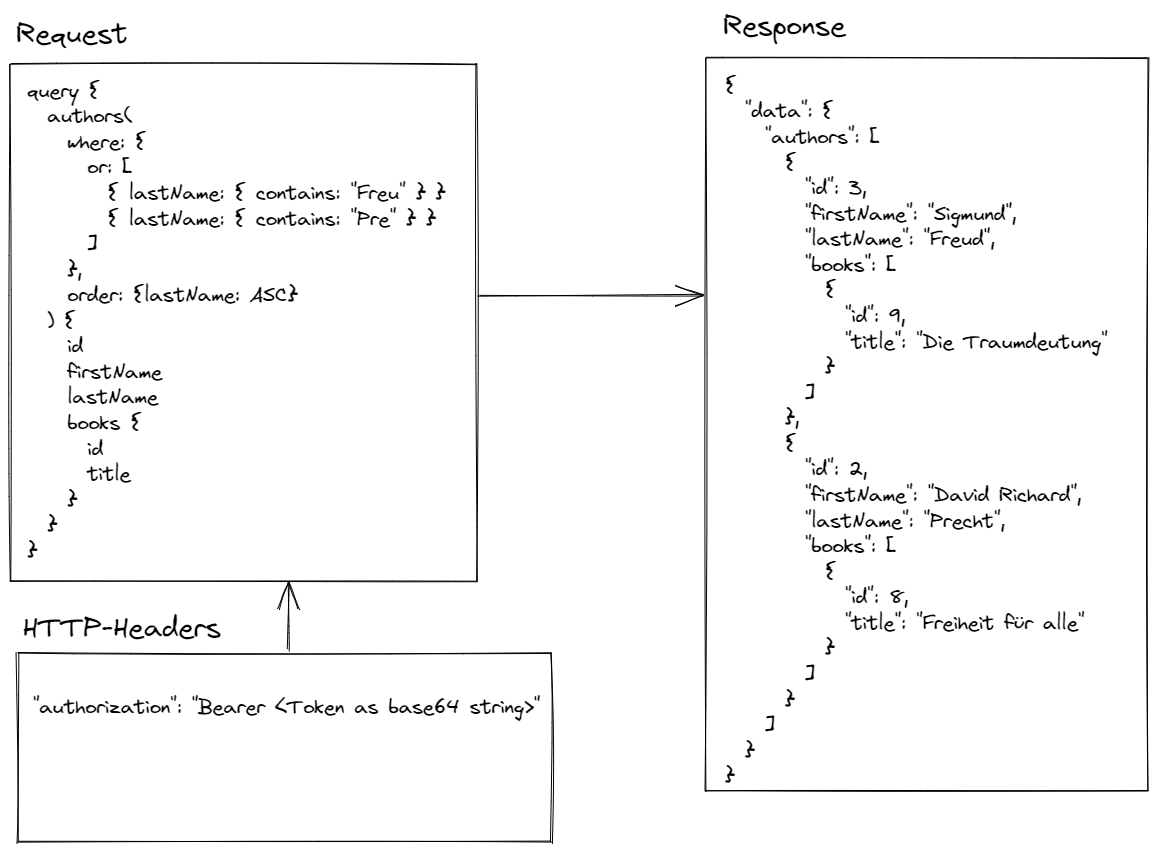
\includegraphics[width=\textwidth]{pics/authors_request.png}
    \caption{Ausführungsreihenfolge Middleware}
\end{figure}

Die obige Abbildung zeigt eine Query, welche alle Autoren mittels dem Feld \textit{authors} abfrägt.
Dabei sollen nur jene Autoren zurückgegeben werden deren Nachname entweder "Freu" oder "Pre" enthält.
Weiters werden die Autoren nach ihrem Nachnamen sortiert.
Bei der Antwort des GraphQL-Service ist zu sehen, dass dieser die Daten genau in jenem Format zurückgibt, in dem sie angefragt worden sind.
Mittles HTTP-Parametern wurde der für die Authentifizierung notwendige \textit{JWT-Token} mitübermittelt.
\newline

Die oben abgebildete Anfrage hat am Server folgende Abfrage an die Datenbank ausgelöst:
\begin{JsCode}
SELECT [a].[Id], [a].[FirstName], [a].[LastName], [t].[Id], [t].[Title], [t].[AuthorsId], [t].[BooksId]
FROM [Authors] AS [a]
LEFT JOIN (
    SELECT [b].[Id], [b].[Title], [a0].[AuthorsId], [a0].[BooksId]
    FROM [AuthorBook] AS [a0]
    INNER JOIN [Books] AS [b] ON [a0].[BooksId] = [b].[Id]
) AS [t] ON [a].[Id] = [t].[AuthorsId]
WHERE ((@__p_0 LIKE N'') OR (CHARINDEX(@__p_0, [a].[LastName]) > 0)) OR ((@__p_1 LIKE N'') OR (CHARINDEX(@__p_1, [a].[LastName]) > 0))
ORDER BY [a].[LastName], [a].[Id], [t].[AuthorsId], [t].[BooksId]
\end{JsCode}

Dieses SQL-Statement verdeutlicht, dass nur die tatsächlich abgefragten Daten in der Datenbank selektiert wurden.

\section{Mutations}
Mutations werden wie bereits erwähnt für schreibende Zugriffe auf den GraphQL-Service verwendet.
In den folgenden Abschnitten wird die Umsetzung einer Mutation für das Bearbeiten eines bereits bestehenden Buches erläutert.
Dabei wird auf das Generieren des Schemas zur Laufzeit als auch der Zugriff auf die Datenbank mittels der Geschäftslogik erläutert.

\myparagraph{Generierung Schema}
Damit ein Client die Möglichkeit hat, auf eine Mutation zuzugreifen, muss der Wurzeloperation im Schema das gewünschte Feld hinzugefügt werden.
Dabei wird, wie bereits bei der Implementierung der Query, die Pure-Code-First-Vorgehensweise angewendet.
\newline
Im folgenden Code wird die Wurzeloperation Mutation um ein Feld \textit{updateBook} erweitert.
Dabei werden nur Benutzern mit den Rollen Admin oder Bibliothekar die Ausführung gestattet.
Als Übergabeparameter bekommt die Funktion das DTO BookUpateInput.
Der Resolver BookResolver kümmert sich dabei um Ausführung der Operation.

\begin{JsCode}
public class BookUpdateInput: InputObjectType<BookUpdate> {
    protected override void Configure(IInputObjectTypeDescriptor<BookUpdate> descriptor) {
        descriptor.Field(f => f.Authors).Type<ListType<NonNullType<IntType>>>();
    }
}

public class BookMutation: ObjectTypeExtension<Mutation>{
    protected override void Configure(IObjectTypeDescriptor<Mutation> descriptor) {
        descriptor.Field("updateBook")
            .Authorize(new [] {"Admin", "Librarian"})
            .Argument("input", a => a.Type<NonNullType<BookUpdateInput>>())
            .ResolveWith<BookResolver>(r => r.UpdateBook(default, default))
            .Type<BookType>();
    }
}
\end{JsCode}

Der obige Code hat die Generierung des folgenden Schemas zur Folge:
\begin{JsCode}
type mutation{
    updateBook(input: BookUpdateInput!): Book @authorize(roles: [ "Admin", "Librarian" ], apply: BEFORE_RESOLVER)
}

type Book {
  title: String!
  authors: [Author!]!
  reviews: [Review!]!
  id: Int!
}

type Author {
  firstName: String!
  lastName: String!
  books: [Book!]!
  id: Int!
}

type Review {
  userId: Int!
  user: User!
  bookId: Int!
  book: Book!
  rating: Int!
  id: Int!
}

type User {
  firstName: String!
  lastName: String!
  email: String!
  roles: [Role!]!
  reviews: [Review!]!
  id: Int!
}

type Role {
  name: String!
  users: [User!]!
  id: Int!
}

input BookUpdateInput {
  authors: [Int!]
  id: Int!
  title: String!
}
\end{JsCode}

Im generierten Schema ist zu erkennen, dass der Typ \textit{Book} alle Typen, die dieser explizit oder implizit referenziert, generiert wurden.
Desweiteren wurde die Wurzeloperation Mutation durch das Feld updateBook erweitert.
Das Feld hat eine \textit{@authorize}-Direktive, welche nur Benutzern mit den Rollen Admin oder Bibliothekar Zugriff gewährt.
Weiters wurde das Input-Objekt \textit{BookUpdateInput} generiert.
\newline

Das Input-Objekt \textit{BookUpateInput} wurde wie folgt deklariert:
\begin{JsCode}
public class BookUpdateInput: InputObjectType<BookUpdate> {

    protected override void Configure(IInputObjectTypeDescriptor<BookUpdate> descriptor) {
        descriptor.Field(f => f.Authors).Type<ListType<NonNullType<IntType>>>();
    }
}

public class BookUpdate {
    public int Id { get; set; }
    public string Title { get; set; }
    public ICollection<int> Authors { get; set; }
}
\end{JsCode}

Bei der Definition des Input-Objekts \textit{BookUpdateInput} bietet die Methode \textit{Configure} der Basisklasse \textit{ObjectType} wiederum die Möglichkeit, genauere Definitionen vorzunehmen.
Im obigen Quelltextausschnitt ist ersichtlich, dass das Feld \textit{authors} eine Liste mit \textit{Int}-Objekten enthält, die nicht \textit{null} sein dürfen.
\newline

Anders als die im Datenbankschema beschriebene Entität Book hält das Input-Objekt BookUdpateInput keine Liste des Typs Author, sondern nur eine Liste von \textit{Int}-Werten, welche die IDs widerspiegeln.
Mit dieser Vorgehensweise wird einer zyklischen Abhängigkeit vorgebeugt, denn sonst würden die Bücher Autoren referenzieren, welche wiederum Bücher referenzieren und das wiederholt sich endlos.
Um diese \textit{DTOs} wieder zu Domänenklassen umzuwandeln, müssen diese auf Datenübertragungsklassen abgebildet werden.
Dafür wird im Prototyp die Bibliothek \textit{AutoMapper} verwendet.

Im folgenden Quelltextausschnitt wird \textit{BookUpdateInput} wieder zu \textit{Book} umgewandelt:
\begin{JsCode}
public class BookProfile : Profile {
    public BookProfile() {
        CreateMap<BookUpdate, Book>()
            .ForMember(
            dest => dest.Authors,
            opt => opt.MapFrom(src => src.Authors.Select(id => new Author { Id = id })));
    }

}
\end{JsCode}

Zum Vergleich hier noch die Klasse Book, welche das Domänenobjekt Book darstellt und von \textit{BaseEntity} ableitet und damit eine \textit{Id} erbt.

\begin{JsCode}
public class Book: BaseEntity {
    public string Title { get; set; }
    public List<Author> Authors { get; set; } = new List<Author>();
    public List<Review> Reviews { get; set; } = new List<Review>();
}
\end{JsCode}
\pagebreak
\myparagraph{Ausführung und Ergebnis}

\begin{figure}[H]
    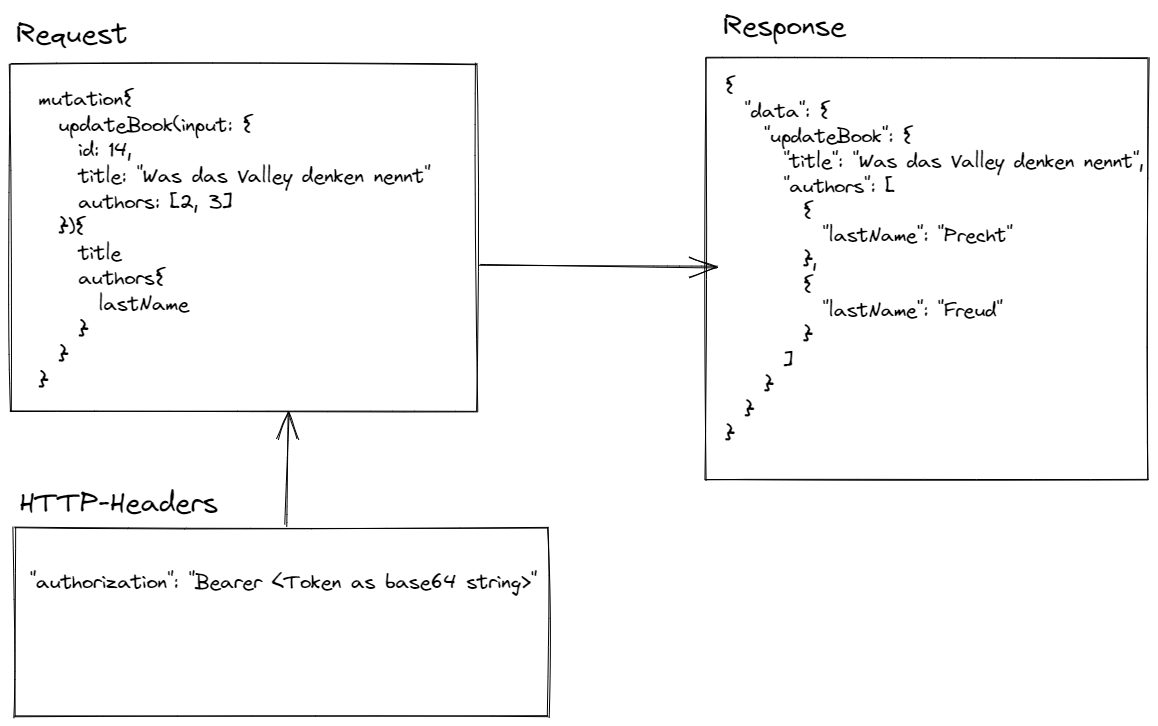
\includegraphics[width=\textwidth]{pics/execution_mutation.png}
    \caption{Schemadefinition}
\end{figure}

In dieser Abbildung ist die Ausführung des Feldes \textit{updateBook} der Mutation zu sehen.
Der Anfrage muss als HTTP-Header ein \textit{JWT-Token} übergeben werden, um zu überprüfen, ob der ausführende Benutzer genügend Rechte hat.
Die Antwort des GraphQL-Service entspricht dabei wiederum genau dem Schema, welches in der Query der Anfrage angegeben wurde.


\section{Subscriptions}
Subscriptions werden wie bereits erwähnt verwendet, um bidirektionale Kommunikation zwischen dem Client und Server zu ermöglichen.
Dabei registriert sich der Client auf Events, welche vom Server ausgelöst werden, und bekommt dadurch in Echtzeit Updates.
HotChocolate realisiert Subscriptions mittels WebSockets.
HotChocolate bietet dabei zwei Subscription-Provider: \textit{In-Memory} und \textit{Redis}.
Für den Prototypen wurde dabei die \textit{In-Memory} Version verwendet.

\myparagraph{Subscription über Event benachrichtigen}
Um eine Subscription über ein ausgeführtes Event zu benachrichtigen, stellt HotChocolate den ITopicEventSender und den ITopicEventReceiver zur Verfügung.
Diese Interfaces sind Abstraktionen der Funktionalitäten des Subscription-Providers.
Diese Abstraktion ermöglicht es dem Entwickler, den Subscription-Provider je nach Bedarf, zu einem späteren Zeitpunkt beliebig auszutauschen.
Um nun eine Subscription von einem Event zu benachrichtigen, muss folgende Methode implementiert werden:
\begin{JsCode}
public async Task<Book> CreateBook([Service] IBookService bookService, BookCreate input,[Service] ITopicEventSender sender) {
    var book = await bookService.AddAsync(mapper.Map<Book>(input));
    await sender.SendAsync("bookAdded", book);
    return book;
}
\end{JsCode}

In Zeile 3 des obigen Quelltextausschnittes wird mittels dem \textit{ITopicEventSender} der \textit{ITopicEventReceiver} von dem neu erstelltem Buch notifiziert.
Auf die Verwendung des \textit{ITopicEventReceiver} wird in der folgenden Implementierung einer Subscription, welche auf die Erstellung eines Buches wartet, näher eingegangen:

\myparagraph{Schemagenerierung}
Für die Generierung des Schemas wird der Pure-Code-First-Ansatz von GraphQL verwendet.
Die Wurzeloperationen Subscription wird dabei um ein Feld \textit{bookAdded} erweitert.
Die Umsetzung ist dabei in folgendem Quelltextausschnitt ersichtlich:

\begin{JsCode}
public class BookSubscription: ObjectTypeExtension<Subscription> {
    protected override void Configure(IObjectTypeDescriptor<Subscription> descriptor) {
        descriptor
        .Field("bookAdded")
        .Type<BookType>()
        .Resolve(context => context.GetEventMessage<Book>())
        .Subscribe(async context => {
            var receiver = context.Service<ITopicEventReceiver>();
            return await receiver.SubscribeAsync<string, Book>("bookAdded");
        });
    }
}    
\end{JsCode}
In Zeile 9 des obigen Quelltextausschnittes ist ersichtlich, dass der \textit{ITopicEventReceiver} auf eine Benachrichtigung durch den \textit{ITopicEventSender} wartet.

Der oben angeführte Code generiert folgendes Schema:
\begin{JsCode}
type subscription{
    bookAdded: Book
}

type Book {
  title: String!
  authors: [Author!]!
  reviews: [Review!]!
  id: Int!
}

type Author {
  firstName: String!
  lastName: String!
  books: [Book!]!
  id: Int!
}

type Review {
  userId: Int!
  user: User!
  bookId: Int!
  book: Book!
  rating: Int!
  id: Int!
}

type User {
  firstName: String!
  lastName: String!
  email: String!
  roles: [Role!]!
  reviews: [Review!]!
  id: Int!
}

type Role {
  name: String!
  users: [User!]!
  id: Int!
}
\end{JsCode}

\myparagraph{Ausführung und Ergebnis}
Auf den Verbindungsaufbau von Subscriptions wurde bereits in Abschnitt 3.7 eingegangen.
Das folgende Bild zeigt das Ergebnis einer Subscription, welche von der Erstellung eines Buches notifiziert wurde.

\begin{figure}[H]
    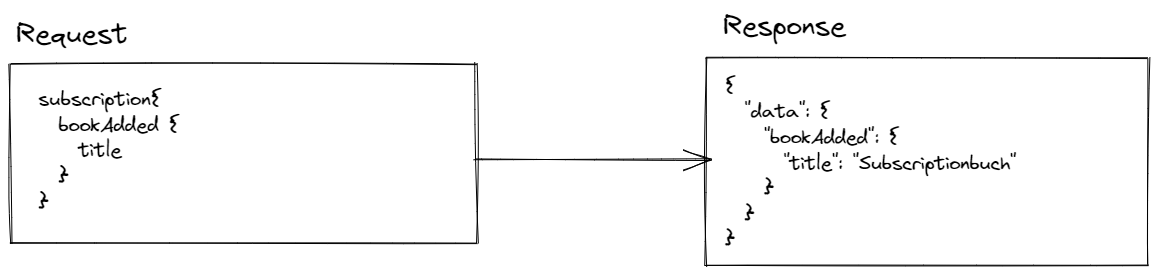
\includegraphics[width=\textwidth]{pics/bookSubscription.png}
    \caption{Subscription welche von der Erstellung eines Buches benachrichtigt wird.}
\end{figure}

\section{Authentifizierung und Autorisierung}
Als Authentifizierung wird jener Vorgang bezeichnet, mit dem die Identität eines Benutzers festgestellt wird.
Die Autorisierung wiederum ermittelt, ob ein Benutzer die erforderlichen Rechte hat, um auf eine bestimmte Ressource zugreifen zu können.
Wie im Anwendungsszenario bereits beschrieben, gibt es im System drei Rollen für Benutzer: \textit{User}, \textit{Librarian} und \textit{Admin}.
Jede Rolle kann nur auf für Sie freigegebene Ressourcen zugreifen.
\newline

Die Authentifizierung und Autorisierung für den Prototyp wird mit \textit{JWT-Tokens} und der Zuhilfenahme der \textit{ASP.NET Core-Authentifizierung} umgesetzt.
Die folgenden Abbildungen beschreiben die Rollen und die Ressourcen, auf die sie Zugriff haben.
Grüne Felder bedeuten dabei, dass auch Benutzer ohne valides \textit{JWT-Token} Zugriff auf diese Ressource haben.
Das gelbe Feld \glqq Einloggen" kann nur nach einer bereits erfolgten Registrierung aufgerufen werden.
Rote Felder wiederum verlangen ein valides \textit{JWT-Token} und sind an die Rolle des aufrufenden Benutzers gebunden.

\begin{figure}[H]
    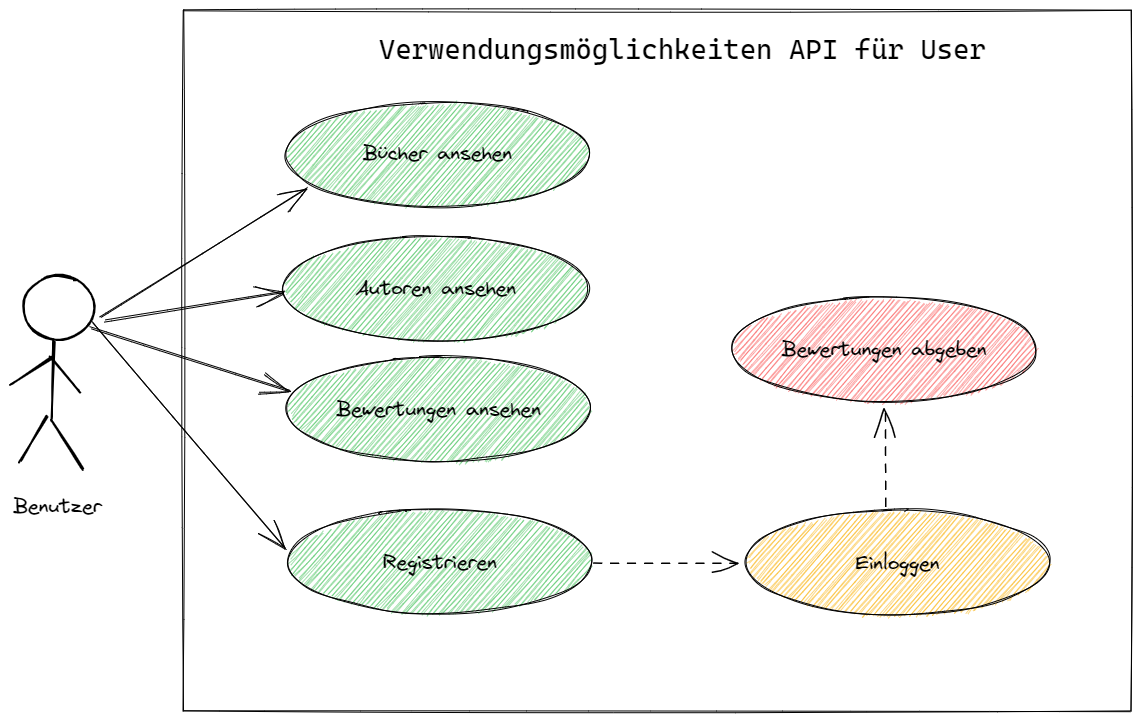
\includegraphics[width=\textwidth]{pics/UseCaseUser.png}
    \caption{Rechte der Rolle \textit{User}.}
\end{figure}

\begin{figure}[H]
    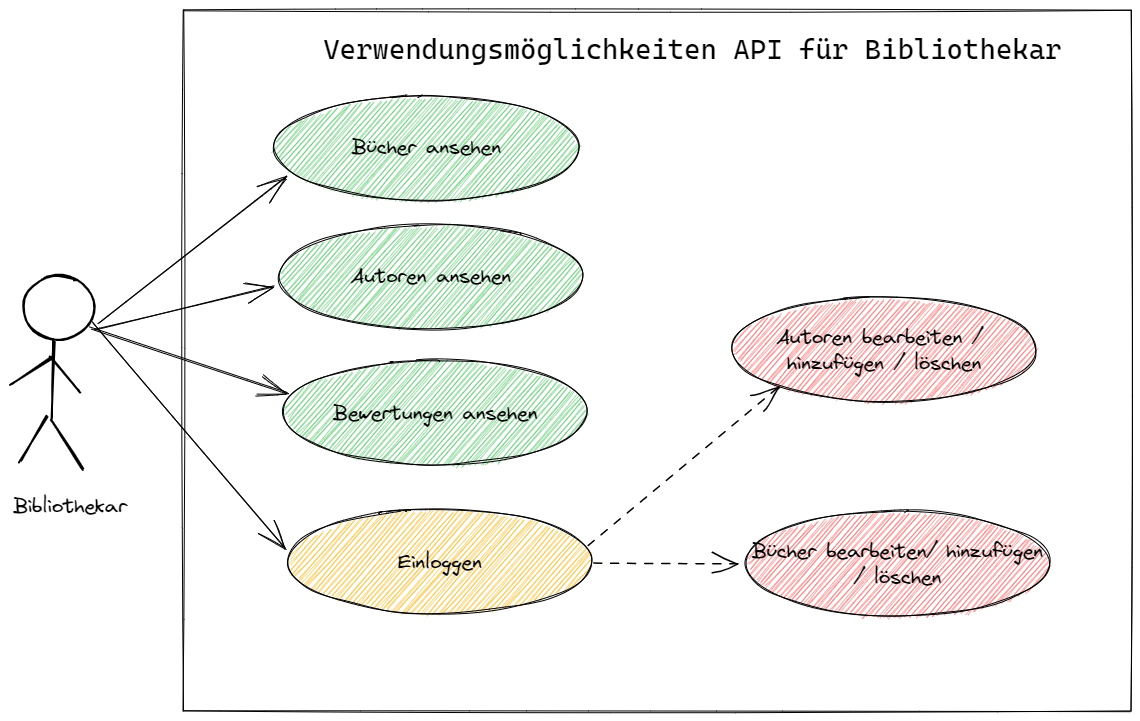
\includegraphics[width=\textwidth]{pics/UseCaseLibrarian.png}
    \caption{Rechte der Rolle \textit{Librarian}.}
\end{figure}

\begin{figure}[H]
    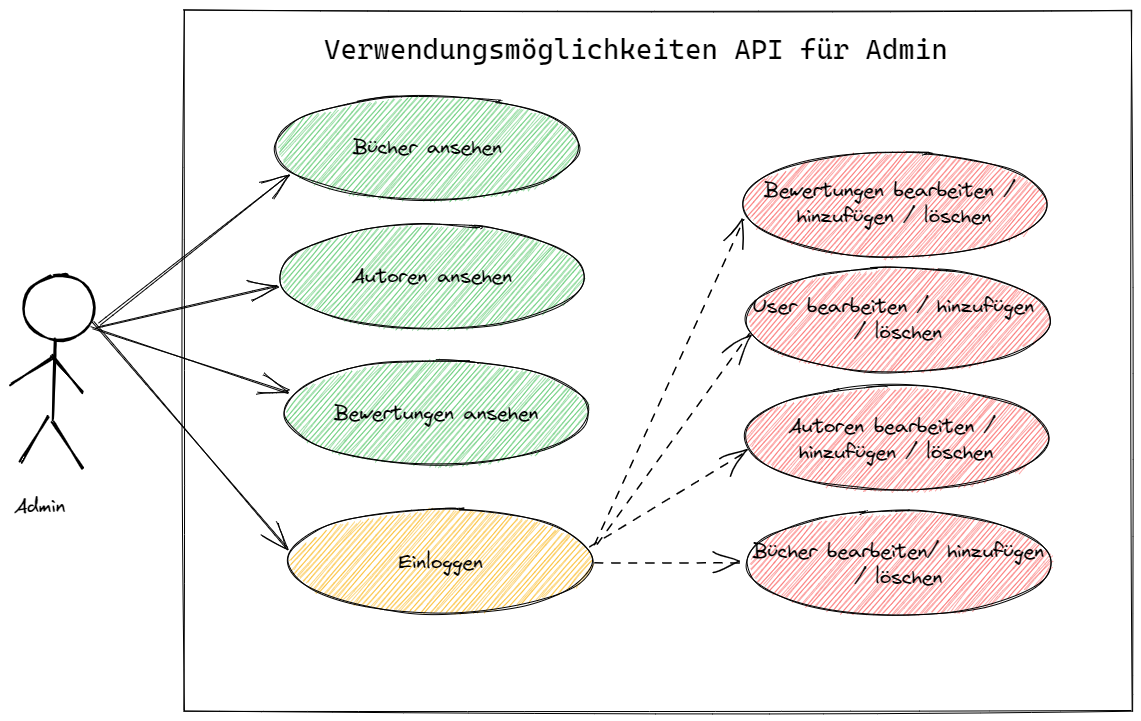
\includegraphics[width=\textwidth]{pics/UseCaseAdmin.png}
    \caption{Rechte der Rolle \textit{Admin}.}
\end{figure}

\myparagraph{Generierung JWT-Token}
Um die Authentifizierung mittels JWT-Token zu ermöglichen, muss diese Authentifizierungsform erst registriert werden. %TODO anderes wort für registrieren, aber gibt es glaube ich nicht
Diese Registrierung erfolgt, wie in .NET üblich, im \textit{WebApplicationBuilder}.

\begin{JsCode}
builder.Services.AddAuthentication(JwtBearerDefaults.AuthenticationScheme)
.AddJwtBearer(options => {
    var tokenSettings = configuration.GetSection("JWT").Get<TokenSettings>();
    options.TokenValidationParameters = new TokenValidationParameters {
        ValidIssuer = tokenSettings.Issuer,
        ValidateIssuer = true,
        ValidAudience = tokenSettings.Audience,
        ValidateAudience = true,
        IssuerSigningKey = new SymmetricSecurityKey(
                                Encoding.UTF8.GetBytes(tokenSettings.Key)),
        ValidateIssuerSigningKey = true
    };
});
\end{JsCode}

Im obigen Code ist zu sehen, dass dem Server, auf dem der GraphQL-Service läuft, eine JWT-Token-Authentifizierung hinzugefügt wird.
Hierzu wurde eine Klasse \textit{TokenSettings} erstellt, welche den \textit{Issuer}, die \textit{Audience} und den \textit{Key}, welche die benötigten Daten aus der \textit{appsettings.json} liest, bereitstellt.
\newline

% Nachdem die zu verwendende Authentifizierungsmethode am Server registriert ist, ist es notwendig die Logik für die Erstellung eines Tokens zu implementieren.
Nach der Registrierung der zu verwendenden Authentifizierungsmethode erfolgt die eigentliche Generierung des Tokens.
Diese wurde im \textit{AuthService} in der Methode \textit{Login} umgesetzt.
Diese Methode erhält einen Benutzernamen und ein Passwort als Übergabeparameter.
Hervorzuheben ist dabei, dass der Login als Mutation umgesetzt wurde.
Zum jetzigen Zeitpunkt finden keine schreibenden Operationen in dieser Methode statt.
Login-Operationen beinhalten aber oftmals das Speichern des letzten erfolgreichen Logins, weswegen für die Implementierung eine Mutation gewählt wurde.
\newline

Im folgenden Quelltextausschnitt wird ein JWT-Token, bei übereinstimmenden User-Credentials, generiert.

\begin{JsCode}
public async Task<string> Login(string email, string password) {
   var user = await userRepository.GetFirstAsync(user => user.Email.Equals(email), user => user.Roles);
   if (user is not null&&BCrypt.Net.BCrypt.Verify(password, user.Password)){
       var securtityKey = new SymmetricSecurityKey(Encoding.UTF8.GetBytes(tokenSettings.Key));
   
       var credentials = new SigningCredentials(securtityKey, SecurityAlgorithms.HmacSha256);
   
       var claims = new List<Claim>();
   
       claims.Add(new Claim("FirstName", user.FirstName));
       claims.Add(new Claim("LastName", user.LastName));
       claims.Add(new Claim("Email", user.Email));
       if (user.Roles?.Count > 0) {
           foreach (var role in user.Roles) {
               claims.Add(new Claim(ClaimTypes.Role, role.Name));
           }
       }
   
       var jwtSecurityToken = new JwtSecurityToken(
           issuer: tokenSettings.Issuer,
           audience: tokenSettings.Audience,
           expires: DateTime.Now.AddDays(1),
           signingCredentials: credentials,
           claims: claims
       );
   
       return new JwtSecurityTokenHandler().WriteToken(jwtSecurityToken);
   }

return "";
}
\end{JsCode}

Der obige Code beinhaltet die Überprüfung der vom Client übergebenen Benutzerdaten.
Stimmen diese mit jenen in der Datenbank überein, so wird ein JWT-Token generiert.
Der Token beinhaltet dabei folgende Daten des Benutzers: \textit{FirstName}, \textit{LastName}, \textit{Email} und die zugewiesenen Rollen.

\myparagraph{Verwendung Authentifizierung und Autorisierung}
Um ein Feld einer Query, Mutation oder Subscription nun abzusichern, muss man die Field-Middleware Authentifizierung bei dem jeweiligen Feld aktivieren.
% Mit Pure-Code-First funktioniert das wie im folgenden Code-Beispiel abgebildet:
Mit der Pure-Code-First Methode von HotChocolate wird die Konfiguration in der \textit{Configure} Methode des jeweiligen \textit{ObjectType} abgebildet.

\begin{JsCode}
public class AuthorQuery: ObjectType<Query> {
    protected override void Configure(IObjectTypeDescriptor<Query> descriptor) {
        descriptor.Field("authors")
            .ResolveWith<AuthorResolver>(r => r.Authors())
            .Authorize()
            .Type<ListType<NonNullType<AuthorType>>>();
    }
}
\end{JsCode}

In dem oben stehenden Code wird festgelegt, dass ein User ein valides \textit{JWT-Token} an den Service übergeben muss, um Zugriff auf die Ressource zu haben.
Im Umkehrschluss bedeutet dies, dass jeder Benutzer des Systems, wenn er angemeldet ist, Zugriff auf diese Ressource hat.
\newline

\section{1 + n Problem}
Die Definition dieses Problems wurde im Abschnitt 3.8 erläutert.
Dieser Abschnitt implementiert eine Lösung des 1 + n Problems mittels eines DataLoaders, welcher von HotChoclate zur Verfügung gestellt wird.
\newline

% Die folgende Abfrage ermöglicht es dem Client, zwei Autoren in einer Abfrage, vom GraphQL-Service abzufragen.
Die folgende Abfrage ermöglicht es dem Client, die Daten von zwei Autoren mittels einer GraphQL-Abfrage zu ermitteln.
\begin{JsCode}
query {
    a: authorByDataLoader(id: 1) {
        id
        firstName
        lastName
    }
    
    b: authorByDataLoader(id: 2) {
        id
        firstName
        lastName
    }
}
\end{JsCode}

Das Problem, welches der GraphQL-Service hat, besteht darin, dass der Resolver kein Wissen über die Abfrage-Query als Ganzes hat.
Der Resolver besitzt also nicht die Information, ob er mehrfach parallel aufgerufen wird, um ähnliche oder gleiche Daten aus derselben Datenquelle abzufragen.
Der DataLoader hat die Aufgabe, diese einzelnen Resolveraufrufe in einen einzigen Datenbankzugriff zusammenzuführen.

\myparagraph{Implementierung DataLoader}
In diesem Abschnitte wird ein DataLoader für Autoren implementiert.
Für die Implementierung wird die Pure-Code-First-Vorgehensweise verwendet.
Für die Realsierung sind folgende Schritte erforderlich:
\newline

Um einen DataLoader mit HotChoclate zu implementieren muss eine neue Klasse erstellt werden welche von \textit{BatchDataLoader} ableitet:
\begin{JsCode}
public class AuthorByIdDataLoader : BatchDataLoader<int, Author> {
    private readonly IAuthorService authorService;

    public AuthorByIdDataLoader
        (IBatchScheduler batchScheduler, IAuthorService authorService,
        DataLoaderOptions? options = null) : base(batchScheduler, options)
    {
        this.authorService = authorService;
    }

    protected override async Task<IReadOnlyDictionary<int, Author>> LoadBatchAsync(
        IReadOnlyList<int> keys, CancellationToken cancellationToken)
    {
        return (await authorService.GetAsync(a => keys.Contains(a.Id)))
               .ToDictionary(t => t.Id);
    }
}
\end{JsCode}
In der Methode \textit{LoadBatchAsync} werden alle Autoren, anhand ihrer IDs, von der \textit{GetAsync}-Methode des \textit{AuthorService} selektiert.
Die \textit{GetAsync}-Methode des \textit{AuthorService} erwartet dabei eine Expression.
\newline

Zusätzlich muss im \textit{AuthorResolver} der DataLoader registriert werden:
\begin{JsCode}
public async Task<Author> AuthorByDataLoader(
    int id,
    AuthorByIdDataLoader dataLoader,
    CancellationToken cancellationToken) 
{
    return await dataLoader.LoadAsync(id, cancellationToken);
}
\end{JsCode}

Anschließend muss die \textit{AuthorQuery} in der \textit{Configure}-Methode um das folgende Feld erweitert werden:
\begin{JsCode}
descriptor.Field("authorByDataLoader")
    .UseProjection()
    .ResolveWith<AuthorResolver>(
        g => g.AuthorByDataLoader(default, default, default))
    .Argument("id", a => a.Type<NonNullType<IntType>>())
    .Type<AuthorType>();
\end{JsCode}

% Der DataLoader fügt, die in der oben angeführten Anfrage auf zwei Autoren zu einem Datenbankzugriff zusammen.
Würde die oben angeführte Anfrage ohne DataLoader exekutiert werden, so würde sie in zwei seperaten Datenbankabfragen münden.
Der DataLoader kümmert sich darum, dass daraus eine einzelene Datenbankabfrage wird.
Dafür werden die Daten, nicht wie in Abschnitt 4.7 direkt vom Resolver abgefragt, sondern vom DataLoader.
Dieser kümmert sich darum, dass die einzeln abgefragten Autoren zu einer Liste aus Schlüssel-Wert-Paaren zusammengeführt werden.
Anschließend führt er diese Abfrage mittels des \textit{AuthorService} auf der Datenbank aus.
\newline

Die Implementierung des \textit{AuthorByDataLoader} mündet anschließend in folgendem Datenbankzugriff:
\begin{JsCode}
SELECT [a].[Id], [a].[FirstName], [a].[LastName]
FROM [Authors] AS [a]
WHERE [a].[Id] IN (1, 2)
\end{JsCode}

Wie an diesem SQL-Statement ersichtlich ist, werden die einzelnen Abfragen zu einer zusammengeführt.